\documentclass[9pt]{beamer}

\usepackage[T1]{fontenc}
\usepackage{color}
\usepackage{graphicx}
\usepackage{natbib}
\usepackage{tikz}
\usepackage{xmpmulti}
\usepackage{animate}

\usetheme{Boadilla}

\usefonttheme{professionalfonts}

\title[Apsis Tools]{Apsis - Document Review Platform}
\subtitle{}
\author{Max Callaghan}
\institute[MCC]{
	%
\includegraphics[height=1cm,width=2cm]{/home/max/Pictures/MCC_Logo_RZ_rgb.jpg}
	
\includegraphics[height=1cm,width=2cm]{MCC_Logo_RZ_rgb.jpg}
}

\usetikzlibrary{shapes.geometric, arrows}
\tikzstyle{startstop} = [rectangle, rounded corners, minimum width=2.5cm, minimum height=1cm,text centered, draw=black, text width=2.5cm, fill=red!30]
\tikzstyle{placeholder} = [rectangle, rounded corners, minimum width=2.5cm, minimum height=1cm,text centered, draw=white, text width=2.5cm, fill=red!00]
\tikzstyle{product} = [rectangle, rounded corners, minimum width=2.5cm, minimum height=1cm,text centered, draw=black, text width=2.5cm, fill=cyan!30]
\tikzstyle{process} = [rectangle, minimum width=2cm, text width=2cm, minimum height=1cm, text centered, draw=black, fill=orange!30]
\tikzstyle{person} = [ellipse, minimum width=2cm, text width=2cm, minimum height=1cm, text centered, draw=black, fill=green!30]
\tikzstyle{io} = [trapezium, trapezium left angle=70, trapezium right angle=110, minimum width=1cm, minimum height=1cm, text centered, draw=black, fill=blue!30, inner sep=10]

\tikzstyle{label} = [rectangle, minimum width=0.8cm, minimum height=0.8cm, text centered, draw=black, fill=blue!0, inner sep=3]

\tikzstyle{arrow} = [thick,-,>=stealth]
\tikzstyle{darrow} = [dotted, thick,-,>=stealth]

\newtheorem*{remark}{}

\bibliographystyle{apalike}

\begin{document}
	
\begin{frame}
	\titlepage
\end{frame}

\addtobeamertemplate{frametitle}{}{%
	\begin{tikzpicture}[remember picture,overlay]
	\node[anchor=north east,yshift=2pt] at (current page.north east) {
\includegraphics[height=0.8cm]{MCC_Logo_RZ_rgb.jpg}};
	\end{tikzpicture}}

\begin{frame}{Background}
The exponential growth in literature about climate change raises challenges for environmental assessments:
\begin{columns}
	\begin{column}{0.5\linewidth}
		\begin{figure}
			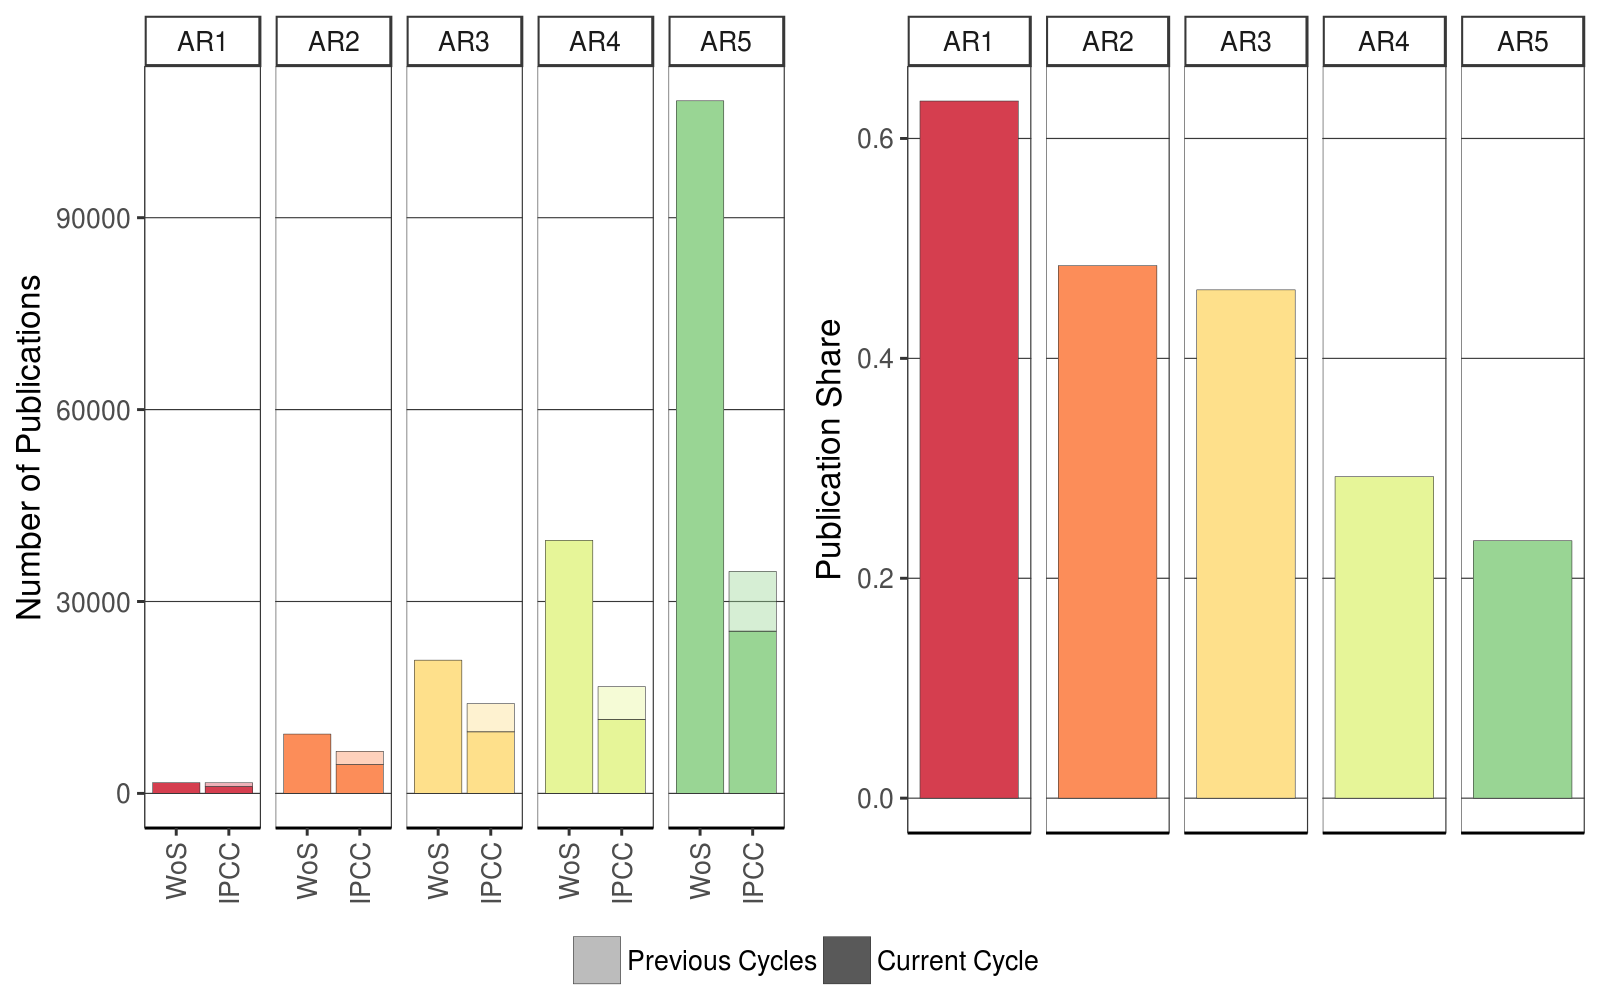
\includegraphics[width=\linewidth]{images/merged_IPCC_spectral}
			\caption{\citep{Minx2017l}}
		\end{figure}
	\end{column}
	\begin{column}{0.5\linewidth}
		\begin{itemize}
			\item<2-> We need to develop ways of being more systematic in engaging with the literature
			\item<3-> We need more research on research results
			\item<4-> We need ways of engaging with large amounts of text
		\end{itemize}
	\end{column}
\end{columns}
\end{frame}

\begin{frame}{Infrastructure Overview}
\begin{center}
	\def\yspace{1.5cm}
	\resizebox{0.9\linewidth}{!}{
		\begin{tikzpicture}[node distance=3cm]
		\node (Data) [startstop] {Data Collection};
		\node (Analysis) [startstop, right of=Data, node distance=6cm] {Analysis};
		\node (Presentation) [startstop, right of=Analysis, node distance=6cm] {Outputs};
		
		\node (WoS) [process, below of=Data, node distance=1.8cm, xshift=-2cm] {WoS};
		\node (Scopus) [process, below of=WoS, node distance=\yspace] {Scopus};
		\node (IPCC) [process, below of=Scopus, node distance=\yspace, fill=orange!10] {IPCC};
		\node (Consolidation) [io, right of=Scopus, node distance=3.5cm] {Consolidation};
		
		\node (Manual) [label, below of=Analysis, node distance=1.8cm, xshift=-1.2cm] {Manual};
		\node (Automatic) [label, below of=Manual, node distance=4.5cm] {Automatic};
		
		
		\node (Review) [process, below of=Analysis, node distance=1.8cm, xshift=1cm] {Systematic Review};
		\node (Scientometric) [process, below of=Review, node distance=\yspace, fill=orange!10] {Scientometric Analysis};
		\node (Text) [process, below of=Scientometric, node distance=\yspace, fill=orange!10] {Other Text Analysis};
		\node (Topics) [process, below of=Text, node distance=\yspace] {Topic Modelling};
		
		\node (Plots) [process, below of=Presentation, node distance=1.8cm, xshift=0cm, fill=orange!10] {Plots};
		\node (Tables) [process, below of=Plots, node distance=\yspace] {Tables};
		\node (Online) [process, below of=Tables, node distance=\yspace] {Online Explorer};	
		
		\draw [arrow, ->] (Manual) -- (Automatic);
		
		\end{tikzpicture}
	}
\end{center}

\end{frame}

%%%%%%%%%%%%%%%%%%%%%%%%%%%%%%%%%%%%%%%%%%%%%%%%%%%%% 
%% Systematic review of NETs



\begin{frame}{Systematic Review - NETs}

For our systematic review of NETs, we wanted to be as systematic in our search, selection and treatment of literature as possible. We developed a system to help us

\begin{columns}
	\begin{column}{0.5\linewidth}
		\begin{itemize}
			\item To search and download (bulk) metadata from Web of Science (WoS) and Scopus
			\item To combine, compare and manage these queries and the documents associated with them
			\item To manage (centrally) the screening of documents by internal and external collaborators
			\item To run analysis based on user-entered tagging of documents and metadata from the WoS/Scopus
		\end{itemize}
	\end{column}
	\begin{column}{0.5\linewidth}
		\begin{figure}
			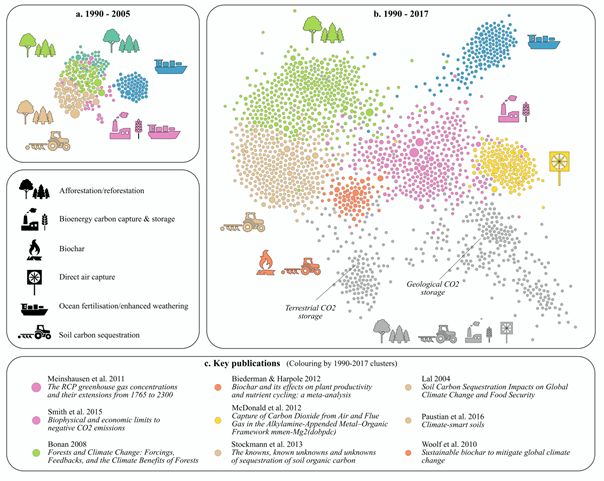
\includegraphics[width=\linewidth]{images/NETs_network}
			\caption{\citep{Minx2017a}}
		\end{figure}
	\end{column}
\end{columns}

\end{frame}


%%%%%%%%%%%%%%%%%%%%%%%%%%%%
%% Sys review process

\begin{frame}{Systematic Review - NETs}
We downloaded over 400 queries, and a team of 18 users reviewed hundreds of documents each.
\begin{figure}
	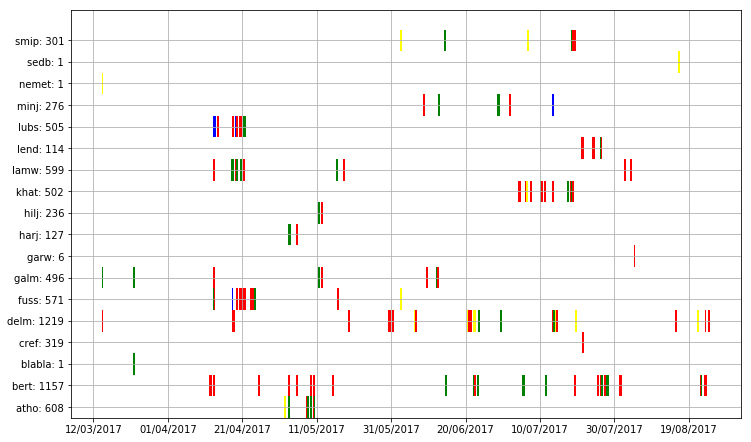
\includegraphics[width=0.8\linewidth]{images/ratings_user_time}
\end{figure}
We used the results to automatically email all authors of relevant documents (over 1000 emails) from which we have received over 100 new documents
\end{frame}


%%%%%%%%%%%%%%%%%%%%%%%%%%%%
%% Website

\begin{frame}{Website}

\url{https://apsis.mcc-berlin.net/scoping}

\end{frame}




%%%%%%%%%%%%%%%%%%%%%%%%%%%%
%% Caveats

\begin{frame}{Caveats}

\begin{block}{Data Collection}<1->

Each time we download a query, we go through a tunnel to PIK (where we have access as Guest Researchers to WoS and Scopus) and instruct the computer to perform a search, and download the results in the maximum chunk size you are allowed (500 or 2000). Both companies prefer that only humans use their website.

\medskip

\textbf{Please therefore do search online, and only download what you need}
\medskip

Longer-term workarounds:
\begin{itemize}
	\item Go through a tunnel to IIASA
	\item Upload Web of Science files directly
\end{itemize}

\end{block}

\begin{block}{In development}<2->
	
	This is lots of pieces of work tied together, written as a side-project to my PhD. I like improving it, and adding more features, but I sometimes break it by accident, and I don't always have time or ability to fix it.
	
\end{block}


\end{frame}

%%%%%%%%%%%%%%%%%%%%%%%%%%%%%%%%%%%%%%%%%%%%%%%%%%%%% 
%% Structure of tool

\begin{frame}{Structure}
	\begin{center}
	\def\yspace{1.5cm}
	\resizebox{0.9\linewidth}{!}{
		\begin{tikzpicture}[node distance=3cm]
		\node<1-> (P) [startstop] {Project};
		\node<1-> (placeholder) [placeholder, right of=P, node distance=8cm] {};
		\node<1-> (placeholder) [placeholder, left of=P, node distance=8cm] {};
		
		% Put users in project
		\node<2-> (U) [startstop, below of=P, node distance=3cm, xshift=-8cm] {User};
		\draw<2-> [arrow] (P) -- (U);
		
		%Do query
		\node<3-> (Q) [startstop, right of=U, node distance=5cm] {Query};
		\draw<3-> [arrow] (U) -- (Q);
		\draw<3-> [arrow] (P) -- (Q);	
		\node<3-> (D) [startstop, below of=Q, node distance=5cm] {Doc};
		\draw<3-> [arrow] (P) -- (Q);
		\draw<3-> [arrow] (D) -- (Q);
		
		% Set up categories and docrels
		\node<4-> (C) [startstop, right of=Q, node distance=2cm, yshift=-1.5cm] {Category};
		\node<4-> (R) [startstop, left of=Q, node distance=5cm, yshift=-3cm] {Relevance};
		\draw<4-> [arrow] (C) -- (Q);
		\draw<4-> [arrow] (R) -- (Q);
		\draw<4-> [arrow] (R) -- (U);
		\draw<4-> [arrow] (P) -- (C);
		
		
		% Go through docs
		\node<5-> (D1) [startstop, right of=D, node distance=0.15cm,yshift=-0.15cm] {Doc};
		\node<5-> (D2) [startstop, right of=D1, node distance=0.15cm,yshift=-0.15cm] {Doc};
		\draw<5-> [arrow] (D) -- (R);
		\draw<5-> [arrow] (D) -- (C);
		%\node<3-> (Presentation) [startstop, right of=Analysis, node distance=6cm] {Presentation};
		
		% Terms
		\node<6-> (Te) [startstop, right of=D2, node distance=9.7cm] {Term};
		\draw<6-> [darrow] (D2) -- (Te);
		
		% Intro topic model
		\node<7-> (M) [startstop, right of=Q, node distance=10cm] {Model};
		\node<7-> (Top) [startstop, right of=Q, node distance=6cm, yshift=-2.5cm] {Topic};
		\draw<7-> [arrow] (M) -- (Q);
		\draw<7-> [arrow] (M) -- (Top);
		
		% doctop, topterm
		\draw<8-> [arrow] (Top) -- (D);
		\draw<8-> [arrow] (Top) -- (Te);
		
		\end{tikzpicture}
	}
\end{center}
\end{frame}

\begin{frame}{Discussion Points}

\begin{itemize}
	\item Is this useful as is?
	\item What features can make it more useful?
	\item Access to MCC hosted site, or package and self-host?
	\item What to do about WoS data access?
\end{itemize}

\end{frame}

\begin{frame}{References}

Code: \url{https://github.com/mcallaghan/tmv}

\medskip

Documentation: \url{https://github.com/mcallaghan/tmv/wiki/Scoping-Documentation} (fairly comprehensive but out of date as of \today)

\medskip

\small
\bibliography{C:/Users/galm/Documents/library/library}
\end{frame}


\end{document}